\documentclass[c]{beamer}

\usepackage{multirow}
\usepackage{pgfplots}
\usepackage{pgfplotstable}
\usepackage{subcaption}
\usepackage{tikz}
\usepackage{xcolor}

\usepgfplotslibrary{fillbetween}
\usepgfplotslibrary{groupplots}
\usepgfplotslibrary{statistics}

\usetikzlibrary{arrows.meta}
\usetikzlibrary{calc}
\usetikzlibrary{shapes}

\usetheme{metropolis}
\author{Esten H{\o}yland Leonardsen}
\title{Detecting individual-level deviations in brain morphology with Layerwise Relevance Propagation}

\definecolor{cb-pink}{HTML}{eeafcf}
\definecolor{cb-orange}{HTML}{e59145}
\definecolor{cb-light-brown}{HTML}{baa066}
\definecolor{cb-blue}{HTML}{3594d6}
\definecolor{cb-green}{HTML}{4dac93}
\definecolor{cb-gray}{HTML}{3a5c7d}
\definecolor{cb-light-purple}{HTML}{b45899}
\definecolor{cb-red-purple}{HTML}{c71555}
\definecolor{cb-brown}{HTML}{840000}
\definecolor{cb-blue-purple}{HTML}{662fa2}

\colorlet{cases-default}{cb-red-purple}
\colorlet{controls-default}{cb-blue}

\newcommand{\N}{5}

\begin{document}
	\begin{frame} % Title
		\maketitle
	\end{frame}

	\begin{frame}{Overview}
		\begin{enumerate}
			\item Build a pipeline for producing phenotype-specific, individual-level deviation-maps from structural MRIs using a CNN and LRP
			\item Validate the methodology in dementia patients
			\item Application (Schizophrenia?)
		\end{enumerate}
	\end{frame}

	\begin{frame}{Layerwise Relevance Propagation recap}
		\begin{center}
			\begin{tikzpicture}					
				\node[circle,draw=black!70, fill=black!70, minimum size=0.65cm, inner sep=2pt] (n00) at (2.5,1.5) {\textcolor{white}{\tiny{0.70}}};
				\node[circle,draw=black!15, fill=black!15, minimum size=0.65cm, inner sep=2pt] (n01) at (2.5,0.75) {\tiny{0.15}};
				\node[circle,draw=black!65, fill=black!65, minimum size=0.65cm, inner sep=2pt] (n02) at (2.5,0) {\textcolor{white}{\tiny{0.65}}};
				\node[circle,draw=white, fill=white, minimum size=0.65cm, inner sep=2pt] (n03) at (2.5,-0.75) {};
				\node[circle,draw=black!30, fill=black!30, minimum size=0.65cm, inner sep=2pt] (n04) at (2.5,-1.5) {\tiny{0.30}};
				
				\node[circle,draw=black!35, fill=black!35, minimum size=0.65cm, inner sep=2pt] (n10) at (4.5,1.125) {\tiny{0.35}};
				\node[circle,draw=black!20, fill=black!20, minimum size=0.65cm, inner sep=2pt] (n11) at (4.5,0.375) {\tiny{0.20}};
				\node[circle,draw=black!40, fill=black!40, minimum size=0.65cm, inner sep=2pt] (n12) at (4.5,-0.375) {\tiny{0.40}};
				\node[circle,draw=black!85, fill=black!85, minimum size=0.65cm, inner sep=2pt] (n13) at (4.5,-1.125) {\textcolor{white}{\tiny{0.85}}};
				
				\node[circle,draw=black!10, fill=black!10, minimum size=0.65cm, inner sep=2pt] (n20) at (6.5,0.75) {\tiny{0.10}};
				\node[circle,draw=black!95, fill=black!95, minimum size=0.65cm, inner sep=2pt] (n21) at (6.5,0) {\textcolor{white}{\tiny{0.95}}};
				\node[circle,draw=black!70, fill=black!70, minimum size=0.65cm, inner sep=2pt] (n22) at (6.5,-0.75) {\textcolor{white}{\tiny{0.70}}};
				
				\node[circle,draw=black!45, fill=black!45, minimum size=0.65cm, inner sep=2pt, label=right:{\scriptsize{age}}] (n31) at (8.5,0) {\textcolor{white}{\tiny{37.0}}};
				
				\draw[color=black!70,-{Latex[length=0.2cm, width=0.25cm]},line width=0.1cm] (0.5,0) to [out=0,in=190] (n00) {};
				\draw[color=black!15,-{Latex[length=0.2cm, width=0.25cm]},line width=0.1cm] (0.5,0) to [out=0,in=185] (n01) {};
				\draw[color=black!65,-{Latex[length=0.2cm, width=0.25cm]},line width=0.1cm] (0.5,0) to [out=0,in=180] (n02) {};
				\draw[color=white,-{Latex[length=0.2cm, width=0.25cm]},line width=0.1cm] (0.5,0) to [out=0,in=175] (n03) {};
				\draw[color=black!30,-{Latex[length=0.2cm, width=0.25cm]},line width=0.1cm] (0.5,0) to [out=0,in=170] (n04) {};
				
				\node[minimum width=1.5cm, minimum height=1.5cm, inner sep=0pt, draw=black, fill=black] at (-0.1,0.1) {
					\includegraphics[width=1.5cm]{data/slice.png}
				};
				\node[minimum width=1.5cm, minimum height=1.5cm, inner sep=0pt, draw=black, fill=black] at (0,0) {
					\includegraphics[width=1.5cm]{data/slice.png}
				};
				\node[minimum width=1.5cm, minimum height=1.5cm, inner sep=0pt, draw=black, fill=black] at (0.1,-0.1) {
					\includegraphics[width=1.5cm]{data/slice.png}
				};
				
				\draw[color=black!30,-{Latex[length=0.2cm, width=0.25cm]},line width=0.1cm] (n00) to [out=-10,in=170] (n10) {};
				\draw[color=black!70,-{Latex[length=0.2cm, width=0.25cm]},line width=0.1cm] (n00) to [out=-20,in=160] (n11) {};
				\draw[color=black!15,-{Latex[length=0.2cm, width=0.25cm]},line width=0.1cm] (n00) to [out=-30,in=150] (n12) {};
				\draw[color=black!90,-{Latex[length=0.2cm, width=0.25cm]},line width=0.1cm] (n00) to [out=-40,in=140] (n13) {};
				
				\draw[color=white,-{Latex[length=0.2cm, width=0.25cm]},line width=0.1cm] (n01) to [out=10,in=190] (n10) {};
				\draw[color=black!15,-{Latex[length=0.2cm, width=0.25cm]},line width=0.1cm] (n01) to [out=-10,in=170] (n11) {};
				\draw[color=black!85,-{Latex[length=0.2cm, width=0.25cm]},line width=0.1cm] (n01) to [out=-20,in=160] (n12) {};
				\draw[color=black!30,-{Latex[length=0.2cm, width=0.25cm]},line width=0.1cm] (n01) to [out=-30,in=150] (n13) {};
				
				\draw[color=black!50,-{Latex[length=0.2cm, width=0.25cm]},line width=0.1cm] (n02) to [out=20,in=200] (n10) {};
				\draw[color=black!20,-{Latex[length=0.2cm, width=0.25cm]},line width=0.1cm] (n02) to [out=10,in=190] (n11) {};
				\draw[color=black!15,-{Latex[length=0.2cm, width=0.25cm]},line width=0.1cm] (n02) to [out=-10,in=170] (n12) {};
				\draw[color=black!75,-{Latex[length=0.2cm, width=0.25cm]},line width=0.1cm] (n02) to [out=-20,in=160] (n13) {};
				
				\draw[color=white,-{Latex[length=0.2cm, width=0.25cm]},line width=0.1cm] (n03) to [out=30,in=210] (n10) {};
				\draw[color=white,-{Latex[length=0.2cm, width=0.25cm]},line width=0.1cm] (n03) to [out=20,in=200] (n11) {};
				\draw[color=white,-{Latex[length=0.2cm, width=0.25cm]},line width=0.1cm] (n03) to [out=10,in=190] (n12) {};
				\draw[color=white,-{Latex[length=0.2cm, width=0.25cm]},line width=0.1cm] (n03) to [out=-10,in=170] (n13) {};
				
				\draw[color=black!10,-{Latex[length=0.2cm, width=0.25cm]},line width=0.1cm] (n04) to [out=40,in=220] (n10) {};
				\draw[color=black!35,-{Latex[length=0.2cm, width=0.25cm]},line width=0.1cm] (n04) to [out=30,in=210] (n11) {};
				\draw[color=black!50,-{Latex[length=0.2cm, width=0.25cm]},line width=0.1cm] (n04) to [out=20,in=200] (n12) {};
				\draw[color=black!80,-{Latex[length=0.2cm, width=0.25cm]},line width=0.1cm] (n04) to [out=10,in=190] (n13) {};
				
				\draw[color=white,-{Latex[length=0.2cm, width=0.25cm]},line width=0.1cm] (n10) to [out=-10,in=170] (n20) {};
				\draw[color=black!80,-{Latex[length=0.2cm, width=0.25cm]},line width=0.1cm] (n10) to [out=-20,in=160] (n21) {};
				\draw[color=black!15,-{Latex[length=0.2cm, width=0.25cm]},line width=0.1cm] (n10) to [out=-30,in=150] (n22) {};
				
				\draw[color=black!35,-{Latex[length=0.2cm, width=0.25cm]},line width=0.1cm] (n11) to [out=10,in=190] (n20) {};
				\draw[color=black!45,-{Latex[length=0.2cm, width=0.25cm]},line width=0.1cm] (n11) to [out=-10,in=170] (n21) {};
				\draw[color=black!70,-{Latex[length=0.2cm, width=0.25cm]},line width=0.1cm] (n11) to [out=-20,in=160] (n22) {};
				
				\draw[color=white,-{Latex[length=0.2cm, width=0.25cm]},line width=0.1cm] (n12) to [out=20,in=200] (n20) {};
				\draw[color=black!50,-{Latex[length=0.2cm, width=0.25cm]},line width=0.1cm] (n12) to [out=10,in=190] (n21) {};
				\draw[color=black!95,-{Latex[length=0.2cm, width=0.25cm]},line width=0.1cm] (n12) to [out=-10,in=170] (n22) {};
				
				\draw[color=black!15,-{Latex[length=0.2cm, width=0.25cm]},line width=0.1cm] (n13) to [out=30,in=210] (n20) {};
				\draw[color=black!35,-{Latex[length=0.2cm, width=0.25cm]},line width=0.1cm] (n13) to [out=20,in=200] (n21) {};
				\draw[color=white,-{Latex[length=0.2cm, width=0.25cm]},line width=0.1cm] (n13) to [out=10,in=190] (n22) {};
				
				\draw[color=black!85,-{Latex[length=0.2cm, width=0.25cm]},line width=0.1cm] (n20) to [out=-10,in=170] (n31) {};
				
				\draw[color=black!80,-{Latex[length=0.2cm, width=0.25cm]},line width=0.1cm] (n21) to (n31) {};
				
				\draw[color=black!95,-{Latex[length=0.2cm, width=0.25cm]},line width=0.1cm] (n22) to [out=10,in=190] (n31) {};
				
			\end{tikzpicture}\\
			\vspace{0.3cm}
			\begin{tikzpicture}					
					\node[circle,draw=red!70, fill=red!70, minimum size=0.65cm, inner sep=2pt] (n00) at (2.5,1.5) {\textcolor{white}{\tiny{16.0}}};
					\node[circle,draw=white, fill=white, minimum size=0.65cm, inner sep=2pt] (n01) at (2.5,0.75) {};
					\node[circle,draw=red!65, fill=red!65, minimum size=0.65cm, inner sep=2pt] (n02) at (2.5,0) {\textcolor{white}{\tiny{13.0}}};
					\node[circle,draw=white, fill=white, minimum size=0.65cm, inner sep=2pt] (n03) at (2.5,-0.75) {};
					\node[circle,draw=red!30, fill=red!30, minimum size=0.65cm, inner sep=2pt] (n04) at (2.5,-1.5) {\textcolor{white}{\tiny{8.0}}};
					
					\node[circle,draw=red!35, fill=red!35, minimum size=0.65cm, inner sep=2pt] (n10) at (4.5,1.125) {\textcolor{white}{\tiny{7.0}}};
					\node[circle,draw=red!40, fill=red!40, minimum size=0.65cm, inner sep=2pt] (n11) at (4.5,0.375) {\textcolor{white}{\tiny{8.0}}};
					\node[circle,draw=red!50, fill=red!50, minimum size=0.65cm, inner sep=2pt] (n12) at (4.5,-0.375) {\textcolor{white}{\tiny{9.0}}};
					\node[circle,draw=red!35, fill=red!35, minimum size=0.65cm, inner sep=2pt] (n13) at (4.5,-1.125) {\textcolor{white}{\tiny{5.0}}};
					
					\node[circle,draw=red!20, fill=red!20, minimum size=0.65cm, inner sep=2pt] (n20) at (6.5,0.75) {\textcolor{white}{\tiny{7.0}}};
					\node[circle,draw=red!95, fill=red!95, minimum size=0.65cm, inner sep=2pt] (n21) at (6.5,0) {\textcolor{white}{\tiny{19.0}}};
					\node[circle,draw=red!70, fill=red!70, minimum size=0.65cm, inner sep=2pt] (n22) at (6.5,-0.75) {\textcolor{white}{\tiny{11.0}}};
					
					\node[circle,draw=red!80, fill=red!80, minimum size=0.65cm, inner sep=2pt, label=right:{\scriptsize{age}}] (n31) at (8.5,0) {\textcolor{white}{\tiny{37.0}}};
					
					\draw[color=red!70,{Latex[length=0.2cm, width=0.25cm]}-,line width=0.1cm] (0.5,0) to [out=0,in=190] (n00) {};
					\draw[color=white,{Latex[length=0.2cm, width=0.25cm]}-,line width=0.1cm] (0.5,0) to [out=0,in=185] (n01) {};
					\draw[color=red!65,{Latex[length=0.2cm, width=0.25cm]}-,line width=0.1cm] (0.5,0) to [out=0,in=180] (n02) {};
					\draw[color=white,{Latex[length=0.2cm, width=0.25cm]}-,line width=0.1cm] (0.5,0) to [out=0,in=175] (n03) {};
					\draw[color=red!30,{Latex[length=0.2cm, width=0.25cm]}-,line width=0.1cm] (0.5,0) to [out=0,in=170] (n04) {};
	
					\node[minimum width=1.5cm, minimum height=1.5cm, inner sep=0pt, draw=black, fill=white] at (-0.1,0.1) {
						\includegraphics[width=1.48cm]{data/brain_age_explanation.png}
					};
					\node[minimum width=1.5cm, minimum height=1.5cm, inner sep=0pt, draw=black, fill=white] at (0,0) {
						\includegraphics[width=1.48cm]{data/brain_age_explanation.png}
					};
					\node[minimum width=1.5cm, minimum height=1.5cm, inner sep=0pt, draw=black, fill=white] at (0.1,-0.1) {
						\includegraphics[width=1.48cm]{data/brain_age_explanation.png}
					};
					
					\draw[color=red!30,{Latex[length=0.2cm, width=0.25cm]}-,line width=0.1cm] (n00) to [out=-10,in=170] (n10) {};
					\draw[color=red!70,{Latex[length=0.2cm, width=0.25cm]}-,line width=0.1cm] (n00) to [out=-20,in=160] (n11) {};
					\draw[color=red!15,{Latex[length=0.2cm, width=0.25cm]}-,line width=0.1cm] (n00) to [out=-30,in=150] (n12) {};
					\draw[color=red!90,{Latex[length=0.2cm, width=0.25cm]}-,line width=0.1cm] (n00) to [out=-40,in=140] (n13) {};
					
					\draw[color=white,{Latex[length=0.2cm, width=0.25cm]}-,line width=0.1cm] (n01) to [out=10,in=190] (n10) {};
					\draw[color=white,{Latex[length=0.2cm, width=0.25cm]}-,line width=0.1cm] (n01) to [out=-10,in=170] (n11) {};
					\draw[color=white,{Latex[length=0.2cm, width=0.25cm]}-,line width=0.1cm] (n01) to [out=-20,in=160] (n12) {};
					\draw[color=white,{Latex[length=0.2cm, width=0.25cm]}-,line width=0.1cm] (n01) to [out=-30,in=150] (n13) {};
					
					\draw[color=red!50,{Latex[length=0.2cm, width=0.25cm]}-,line width=0.1cm] (n02) to [out=20,in=200] (n10) {};
					\draw[color=red!20,{Latex[length=0.2cm, width=0.25cm]}-,line width=0.1cm] (n02) to [out=10,in=190] (n11) {};
					\draw[color=red!15,{Latex[length=0.2cm, width=0.25cm]}-,line width=0.1cm] (n02) to [out=-10,in=170] (n12) {};
					\draw[color=red!75,{Latex[length=0.2cm, width=0.25cm]}-,line width=0.1cm] (n02) to [out=-20,in=160] (n13) {};
					
					\draw[color=white,{Latex[length=0.2cm, width=0.25cm]}-,line width=0.1cm] (n03) to [out=30,in=210] (n10) {};
					\draw[color=white,{Latex[length=0.2cm, width=0.25cm]}-,line width=0.1cm] (n03) to [out=20,in=200] (n11) {};
					\draw[color=white,{Latex[length=0.2cm, width=0.25cm]}-,line width=0.1cm] (n03) to [out=10,in=190] (n12) {};
					\draw[color=white,{Latex[length=0.2cm, width=0.25cm]}-,line width=0.1cm] (n03) to [out=-10,in=170] (n13) {};
					
					\draw[color=red!10,{Latex[length=0.2cm, width=0.25cm]}-,line width=0.1cm] (n04) to [out=40,in=220] (n10) {};
					\draw[color=red!35,{Latex[length=0.2cm, width=0.25cm]}-,line width=0.1cm] (n04) to [out=30,in=210] (n11) {};
					\draw[color=red!50,{Latex[length=0.2cm, width=0.25cm]}-,line width=0.1cm] (n04) to [out=20,in=200] (n12) {};
					\draw[color=red!80,{Latex[length=0.2cm, width=0.25cm]}-,line width=0.1cm] (n04) to [out=10,in=190] (n13) {};
					
					\draw[color=white,{Latex[length=0.2cm, width=0.25cm]}-,line width=0.1cm] (n10) to [out=-10,in=170] (n20) {};
					\draw[color=red!80,{Latex[length=0.2cm, width=0.25cm]}-,line width=0.1cm] (n10) to [out=-20,in=160] (n21) {};
					\draw[color=red!15,{Latex[length=0.2cm, width=0.25cm]}-,line width=0.1cm] (n10) to [out=-30,in=150] (n22) {};
					
					\draw[color=red!35,{Latex[length=0.2cm, width=0.25cm]}-,line width=0.1cm] (n11) to [out=10,in=190] (n20) {};
					\draw[color=red!45,{Latex[length=0.2cm, width=0.25cm]}-,line width=0.1cm] (n11) to [out=-10,in=170] (n21) {};
					\draw[color=red!70,{Latex[length=0.2cm, width=0.25cm]}-,line width=0.1cm] (n11) to [out=-20,in=160] (n22) {};
					
					\draw[color=white,{Latex[length=0.2cm, width=0.25cm]}-,line width=0.1cm] (n12) to [out=20,in=200] (n20) {};
					\draw[color=red!50,{Latex[length=0.2cm, width=0.25cm]}-,line width=0.1cm] (n12) to [out=10,in=190] (n21) {};
					\draw[color=red!95,{Latex[length=0.2cm, width=0.25cm]}-,line width=0.1cm] (n12) to [out=-10,in=170] (n22) {};
					
					\draw[color=red!15,{Latex[length=0.2cm, width=0.25cm]}-,line width=0.1cm] (n13) to [out=30,in=210] (n20) {};
					\draw[color=red!35,{Latex[length=0.2cm, width=0.25cm]}-,line width=0.1cm] (n13) to [out=20,in=200] (n21) {};
					\draw[color=white,{Latex[length=0.2cm, width=0.25cm]}-,line width=0.1cm] (n13) to [out=10,in=190] (n22) {};
					
					\draw[color=red!85,{Latex[length=0.2cm, width=0.25cm]}-,line width=0.1cm] (n20) to [out=-10,in=170] (n31) {};
					
					\draw[color=red!80,{Latex[length=0.2cm, width=0.25cm]}-,line width=0.1cm] (n21) to  (n31) {};
					
					\draw[color=red!95,{Latex[length=0.2cm, width=0.25cm]}-,line width=0.1cm] (n22) to [out=10,in=190] (n31) {};
					
			\end{tikzpicture}
		\end{center}
	\end{frame}
	
	\begin{frame}{Dementia: Dataset} % Full dataset
		\pgfplotstableread[col sep=comma]{data/dementia_dataset/dementia_full.csv}\dementiafull
		
		\colorlet{timepoints}{cb-green}

		\def\xmin{46}
		\def\xmax{99}
		\def\ymin{-1.4}
		\def\ymax{1.2}
		
		\centering
		\begin{tikzpicture}
            \begin{axis}[
                width=1.125\textwidth,
                height=0.75\textwidth,
                xmin=\xmin,
                xmax=\xmax,
                ymin=\ymin,
                ymax=\ymax,
                xtick={55,60,65,70,75,80,85,90,95},
				axis lines=center,
				axis y line=none,
            ]
                \addplot[name path=zero, draw=none] coordinates {(47,0) (97,0)};
                \addplot[name path=fcases, draw=cases-default, very thick] table [x=x, y=F-cases]{\dementiafull};\label{trace:cases}
                \addplot[fill=cases-default, opacity=0.2] fill between [of=zero and fcases];
                \addplot[name path=fcontrols, draw=controls-default, very thick] table [x=x, y=F-controls]{\dementiafull};\label{trace:controls}
                \addplot[fill=controls-default, opacity=0.2] fill between [of=zero and fcontrols];
                \addplot[name path=mcases, draw=cases-default, very thick] table [x=x,y expr=\thisrow{M-cases} * -1]{\dementiafull};
                \addplot[fill=cases-default, opacity=0.2] fill between [of=zero and mcases];
                \addplot[name path=mcontrols, draw=controls-default, very thick] table [x=x,y expr=\thisrow{M-controls} * -1]{\dementiafull};
                \addplot[fill=controls-default, opacity=0.2] fill between [of=zero and mcontrols];
                \node[anchor=south west] at (axis cs: 46, 0.07) {\textbf{FEMALE}};
                \node[anchor=north west] at (axis cs: 46, -0.07) {\textbf{MALE}};
                \node[anchor=south, align=center] (n) at (axis cs: 72.5,-1.2) {n=1440};
                \node[anchor=north,font=\footnotesize] at ($(n.south) + (0,-2.5) $) {\ref{trace:controls} Controls\hspace{0.3cm}\ref{trace:cases} Cases};
            \end{axis}
        \end{tikzpicture}
	\end{frame}
	
	\begin{frame}{Dementia: Dataset} % Sites
		\pgfplotstableread[col sep=comma]{data/dementia_dataset/dementia_addneuromed_GE_MEDICAL_SYSTEMS.csv}\dementiage
		\pgfplotstableread[col sep=comma]{data/dementia_dataset/dementia_addneuromed_PICKER_International_Inc.csv}\dementiapicker
		\pgfplotstableread[col sep=comma]{data/dementia_dataset/dementia_ADNI_15T.csv}\dementiaadnione
		\pgfplotstableread[col sep=comma]{data/dementia_dataset/dementia_ADNI_30T.csv}\dementiaadnithree
		\pgfplotstableread[col sep=comma]{data/dementia_dataset/dementia_AIBL_10.csv}\dementiaaiblone
		\pgfplotstableread[col sep=comma]{data/dementia_dataset/dementia_AIBL_20.csv}\dementiaaibltwo
		\pgfplotstableread[col sep=comma]{data/dementia_dataset/dementia_miriad_15_T_Signa.csv}\dementiamiriad
		\pgfplotstableread[col sep=comma]{data/dementia_dataset/dementia_oasis3_15T.csv}\dementiaoasisone
		\pgfplotstableread[col sep=comma]{data/dementia_dataset/dementia_oasis3_30T.csv}\dementiaoasisthree
		\pgfplotstableread[col sep=comma]{data/dementia_dataset/dementia_Oslo_GE750.csv}\dementiaoslo
		\pgfplotstableread[col sep=comma]{data/dementia_dataset/dementia_timepoints.csv}\dementiatimepoints	
	
		\def\xmin{46}
		\def\xmax{99}
		\def\ymin{-1.3}
		\def\ymax{1.3}
		
	    \begin{figure}
        \newcommand{\scannersubplot}[3]{
            \nextgroupplot[
				    axis lines=center,
				    axis y line=none,
                    xmin=\xmin,
                    xmax=\xmax,
                    ymin=\ymin - 0.25,
                    ymax=\ymax + 0.25,
                    xmajorticks=false,
                    axis line style={-}
			    ]
			        
                    \addplot[name path=zero, draw=none] coordinates {(\xmin,0) (\xmax,0)};
                    \addplot[name path=fcases, draw=cases-default, very thick] table [x=x, y=F-cases]{####1};
                    \addplot[fill=cases-default, opacity=0.2] fill between [of=zero and fcases];
                    \addplot[name path=fcontrols, draw=controls-default, very thick] table [x=x, y=F-controls]{####1};
                    \addplot[fill=controls-default, opacity=0.2] fill between [of=zero and fcontrols];
                    \addplot[name path=mcases, draw=cases-default, very thick] table [x=x,y expr=\thisrow{M-cases} * -1]{####1};
                    \addplot[fill=cases-default, opacity=0.2] fill between [of=zero and mcases];
                    \addplot[name path=mcontrols, draw=controls-default, very thick] table [x=x,y expr=\thisrow{M-controls} * -1]{####1};
                    \addplot[fill=controls-default, opacity=0.2] fill between [of=zero and mcontrols];
                    \node[anchor=south] at (axis cs: 72.5,1) {\tiny{####2}};
                    \node[anchor=north] at (axis cs: 72.5,-1) {\tiny{\textbf{n=####3}}};
        }
        	\begin{tikzpicture}
          	\begin{groupplot}[
  			    group style={
  				    group size=5 by 2,
  				    horizontal sep=0.25cm,
  				    vertical sep=0.25cm
  			    },
  			    height=0.314\textwidth,
  			    width=0.314\textwidth
  		    ]
  		        \scannersubplot{\dementiaoasisthree}{OASIS3 3.0T}{430}
  		        \scannersubplot{\dementiaadnione}{ADNI 1.5T}{300}
  		        \scannersubplot{\dementiaadnithree}{ADNI 3.0T}{266}
  		        \scannersubplot{\dementiaoslo}{Oslo GE750}{210}
  		        \scannersubplot{\dementiaaiblone}{AIBL Site 1}{90}
  		        \scannersubplot{\dementiage}{ANM GE}{72}
  		        \scannersubplot{\dementiamiriad}{MIRIAD}{32}
  		        \scannersubplot{\dementiaaibltwo}{AIBL Site 2}{22}
  		        \scannersubplot{\dementiapicker}{ANM Picker}{10}
  		        \scannersubplot{\dementiaoasisone}{OASIS3 1.5T}{8}
  		    \end{groupplot}
        \end{tikzpicture}
        \end{figure}
	\end{frame}
	
	\begin{frame}{Dementia: Dataset} % Diagnostic criteria
		\centering
	    \begin{tabular}{|c|c|c|}
            \hline
             \textbf{\scriptsize{Dataset}}&\textbf{\scriptsize{Controls}}&\textbf{\scriptsize{Patients}}\\
            \hline
            \scriptsize{AddNeuroMed}&\scriptsize{MMSE $\geq$ 24}&\scriptsize{MMSE $<$ 19}\\
            \hline
            \scriptsize{ADNI}&\scriptsize{Group = CN}&\scriptsize{Group = AD}\\
            \hline
            \scriptsize{AIBL}&\scriptsize{Group = DXNORM}&\scriptsize{Group $\in$ \{DXAD, DXOTHDEM\}}\\
            \hline
            \scriptsize{\textcolor{red}{CADDementia}}&\scriptsize{\textcolor{red}{?}}&\scriptsize{\textcolor{red}{?}}\\
            \hline
            \scriptsize{Demgen}&\scriptsize{-}&\scriptsize{DX $\in$ \{AD, OtherDem, UnspecDem, VaD\}}\\
            \hline
            \scriptsize{MIRIAD}&\scriptsize{Group = Control}&\scriptsize{Group = AD}\\
            \hline
            \scriptsize{OASIS3}&\scriptsize{NORMCOG = 1}&\scriptsize{NORMCOG = 0 \& DEMENTED = 1}\\
            \hline
            \scriptsize{StrokeMRI}&\scriptsize{Group = Control}&\scriptsize{-}\\
            \hline
            \scriptsize{TOP}&\scriptsize{diagnosis = CTRL}&\scriptsize{-}\\
            \hline
        \end{tabular}
	\end{frame}	
	
	\begin{frame}{Dementia: Dataset} % Timepoints
		\pgfplotstableread[col sep=comma]{data/dementia_dataset/dementia_timepoints.csv}\dementiatimepoints
		
		\colorlet{timepoints}{cb-green}
		
		\centering
		\begin{tikzpicture}
            \begin{axis}[
                width=\textwidth,
                height=0.5\textwidth,
                ymin=0,
                ymax=550,
                xtick style={draw=none},
                ytick style={draw=none},
                ylabel=\scriptsize{Number of participants},
                xlabel=\scriptsize{Timepoints},
                every tick label/.append style={font=\scriptsize}
            ]
                \addplot [ybar, bar width=0.9, fill=timepoints] table [x=timepoint, y=count] {\dementiatimepoints};
            \end{axis}
        \end{tikzpicture}
	\end{frame}
	
	\begin{frame}{Dementia: Modelling} % Model
		\vfill
		\centering
		Binary SFCN
		\vfill
	\end{frame}
	
	\begin{frame}{Dementia: Modelling} % Data splitting
		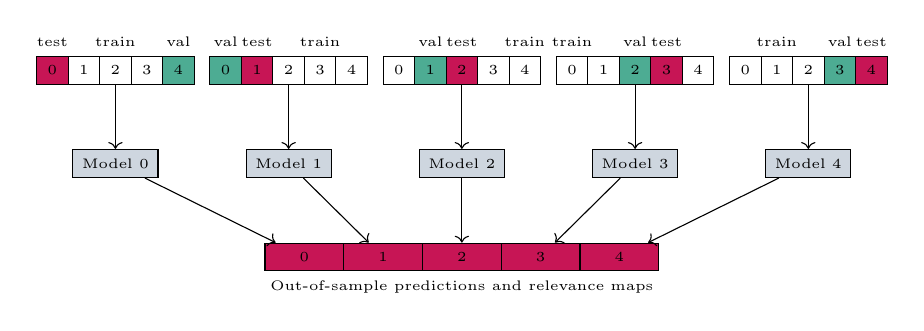
\begin{tikzpicture}
			\newcommand{\width}{0.4}
			\newcommand{\boxwidth}{0.4cm}
			\newcommand{\gap}{\width * 5.5}
			
			\node[
				draw=black,
				minimum width=\boxwidth,
				fill=cb-red-purple,
				label=\tiny{test}
			] at (0*\gap + 0*\width,0) {\tiny{0}};
			\node[
				draw=black,
				minimum width=\boxwidth
			] at (0*\gap + 1*\width,0) {\tiny{1}};
			\node[
				draw=black,
				minimum width=\boxwidth,
				label=\tiny{train}
			] (fold0) at (0*\gap + 2*\width,0) {\tiny{2}};			
			\node[
				draw=black,
				minimum width=\boxwidth
			] at (0*\gap + 3*\width,0) {\tiny{3}};			
			\node[
				draw=black,
				minimum width=\boxwidth,
				fill=cb-green,
				label=\tiny{val}
			] at (0*\gap + 4*\width,0) {\tiny{4}};
			
			\node[
				draw=black,
				minimum width=\boxwidth,
				fill=cb-green,
				label=\tiny{val}
			] at (1*\gap + 0*\width,0) {\tiny{0}};
			\node[
				draw=black,
				minimum width=\boxwidth,
				fill=cb-red-purple,
				label=\tiny{test}
			] at (1*\gap + 1*\width,0) {\tiny{1}};
			\node[
				draw=black,
				minimum width=\boxwidth
			] (fold1) at (1*\gap + 2*\width,0) {\tiny{2}};			
			\node[
				draw=black,
				minimum width=\boxwidth,
				label=\tiny{train}
			] at (1*\gap + 3*\width,0) {\tiny{3}};			
			\node[
				draw=black,
				minimum width=\boxwidth
			] at (1*\gap + 4*\width,0) {\tiny{4}};
			
			\node[
				draw=black,
				minimum width=\boxwidth
			] at (2*\gap + 0*\width,0) {\tiny{0}};
			\node[
				draw=black,
				minimum width=\boxwidth,
				fill=cb-green,
				label=\tiny{val}
			] at (2*\gap + 1*\width,0) {\tiny{1}};
			\node[
				draw=black,
				minimum width=\boxwidth,
				fill=cb-red-purple,
				label=\tiny{test}
			] (fold2) at (2*\gap + 2*\width,0) {\tiny{2}};			
			\node[
				draw=black,
				minimum width=\boxwidth
			] at (2*\gap + 3*\width,0) {\tiny{3}};			
			\node[
				draw=black,
				minimum width=\boxwidth,
				label=\tiny{train}
			] at (2*\gap + 4*\width,0) {\tiny{4}};
			
			\node[
				draw=black,
				minimum width=\boxwidth,
				label=\tiny{train}
			] at (3*\gap + 0*\width,0) {\tiny{0}};
			\node[
				draw=black,
				minimum width=\boxwidth
			] at (3*\gap + 1*\width,0) {\tiny{1}};
			\node[
				draw=black,
				minimum width=\boxwidth,
				fill=cb-green,
				label=\tiny{val}
			] (fold3) at (3*\gap + 2*\width,0) {\tiny{2}};			
			\node[
				draw=black,
				minimum width=\boxwidth,
				fill=cb-red-purple,
				label=\tiny{test}
			] at (3*\gap + 3*\width,0) {\tiny{3}};			
			\node[
				draw=black,
				minimum width=\boxwidth
			] at (3*\gap + 4*\width,0) {\tiny{4}};

			\node[
				draw=black,
				minimum width=\boxwidth
			] at (4*\gap + 0*\width,0) {\tiny{0}};
			\node[
				draw=black,
				minimum width=\boxwidth,
				label=\tiny{train}
			] at (4*\gap + 1*\width,0) {\tiny{1}};
			\node[
				draw=black,
				minimum width=\boxwidth
			] (fold4) at (4*\gap + 2*\width,0) {\tiny{2}};			
			\node[
				draw=black,
				minimum width=\boxwidth,
				fill=cb-green,
				label=\tiny{val}
			] at (4*\gap + 3*\width,0) {\tiny{3}};			
			\node[
				draw=black,
				minimum width=\boxwidth,
				fill=cb-red-purple,
				label=\tiny{test}
			] at (4*\gap + 4*\width,0) {\tiny{4}};
			
			\node[draw=black, fill=cb-gray!25] (model0) at ($ (fold0.south) - (0, 1) $) {\tiny{Model 0}};
			\node[draw=black, fill=cb-gray!25] (model1) at ($ (fold1.south) - (0, 1) $) {\tiny{Model 1}};
			\node[draw=black, fill=cb-gray!25] (model2) at ($ (fold2.south) - (0, 1) $) {\tiny{Model 2}};
			\node[draw=black, fill=cb-gray!25] (model3) at ($ (fold3.south) - (0, 1) $) {\tiny{Model 3}};
			\node[draw=black, fill=cb-gray!25] (model4) at ($ (fold4.south) - (0, 1) $) {\tiny{Model 4}};
			
			\node[draw=black, fill=cb-red-purple, minimum width=1cm, label=below:{\tiny{Out-of-sample predictions and relevance maps}}] (pred2) at ($ (model2.south) - (0, 1) $) {\tiny{2}};
			\node[draw=black, fill=cb-red-purple, minimum width=1cm] (pred1) at ($ (model2.south) - (1, 1) $) {\tiny{1}};
			\node[draw=black, fill=cb-red-purple, minimum width=1cm] (pred0) at ($ (model2.south) - (2, 1) $) {\tiny{0}};
			\node[draw=black, fill=cb-red-purple, minimum width=1cm] (pred3) at ($ (model2.south) - (-1, 1) $) {\tiny{3}};
			\node[draw=black, fill=cb-red-purple, minimum width=1cm] (pred4) at ($ (model2.south) - (-2, 1) $) {\tiny{4}};
			
			\draw[->] (fold0) -- (model0);
			\draw[->] (fold1) -- (model1);
			\draw[->] (fold2) -- (model2);
			\draw[->] (fold3) -- (model3);
			\draw[->] (fold4) -- (model4);
			
			\draw[->] (model0) -- (pred0);
			\draw[->] (model1) -- (pred1);
			\draw[->] (model2) -- (pred2);
			\draw[->] (model3) -- (pred3);
			\draw[->] (model4) -- (pred4);			
		\end{tikzpicture}
	\end{frame}	
	
	\begin{frame}{Dementia: Modelling} % Augmenters
		\centering
	    \begin{tabular}{|c|c|c|}
	        \multicolumn{1}{c}{}&\multicolumn{2}{c}{\scriptsize{Parameterization}}\\
	        \hline
	        \textbf{\scriptsize{Augmentation}}&\textbf{\scriptsize{Light augmenter}}&\textbf{\scriptsize{Heavy augmenter}}\\
	        \hline
	        \scriptsize{Flip}&\scriptsize{0.5,0.0,0.0\textsuperscript{(1)}}&\scriptsize{0.5,0.0,0.0\textsuperscript{(1)}}\\
	        \hline
	        \scriptsize{Shift}&\scriptsize{[-5,5]\textsuperscript{(2)}}&\scriptsize{[-5,5]\textsuperscript{(2)}}\\
	        \hline
	        \scriptsize{Zoom}&\scriptsize{-}&\scriptsize{[-0.05,0.05]\textsuperscript{(2)}}\\
	        \hline
	        \scriptsize{Rotation}&\scriptsize{-}&\scriptsize{[-5,5]\textsuperscript{(2)}}\\
	        \hline
	        \scriptsize{Noise}&\scriptsize{-}&\scriptsize{[0, 0.1]\textsuperscript{(2)}}\\
	        \hline
	        \scriptsize{Intensity}&\scriptsize{-}&\scriptsize{[0, 0.2]\textsuperscript{(2)}}\\
	        \hline
	        \scriptsize{Blur}&\scriptsize{-}&\scriptsize{3\textsuperscript{(3)} (0.2)\textsuperscript{(2)}}\\
	        \hline
	        \scriptsize{\textcolor{red}{Contrast}}&\scriptsize{\textcolor{red}{-}}&\scriptsize{\textcolor{red}{?}}\\
	        \hline
	        \scriptsize{Crop box (size)}&\scriptsize{[0, 50]\textsuperscript{(2)}}&\scriptsize{[0, 50]\textsuperscript{(2)}}\\
	        \hline
	    \end{tabular}\\
	    \vspace{0.2cm}
	    \tiny{(1) Probability of occuring per image per epoch}\\
	    \tiny{(2) Parameter drawn from range per image per epoch}\\
	    \tiny{(3) Fixed kernel size}\\
	\end{frame}	
	
	\begin{frame}{Dementia: Modelling} % Learning rate
		\pgfplotstableread[col sep=comma]{data/dementia_learning_rates/learning_rate_sweep.csv}\dementiasweep
		\pgfplotstableread[col sep=comma]{data/dementia_learning_rates/learning_rates.csv}\dementialr
		
		\centering
		\vspace{0.2cm}
	    \begin{tikzpicture}
            \begin{axis}[
                width=1.06\textwidth,
                height=0.4\textwidth,
                xmode=log,
                ymode=log,
                xmin=0.00001,
                xmax=10,
                ylabel=\scriptsize{Logloss},
                xlabel=\scriptsize{Learning rate},
                ymajorticks=false,
                xlabel=\scriptsize{Prediction},
                every tick label/.append style={font=\scriptsize}
            ]
                \addplot[draw=cb-gray,very thick] table [x=lr, y=loss] {\dementiasweep};
            \end{axis}
        \end{tikzpicture}
        \par\bigskip
        \newcommand{\lrsubplot}[5]{
            \nextgroupplot[
                    xmin=0,
                    xmax=160,
                    ymin=-0.01,
                    ymax=0.11,
                    ymajorticks=####2,
                    xtick pos=bottom,
                    ytick pos=left,
                    ytick={0, 0.02, 0.04, 0.06, 0.08, 0.1},
                    yticklabels={0, 0.02, 0.04, 0.06, 0.08, 0.1},
                    title=\scriptsize{####3},
                    xlabel=\scriptsize{####4},
                	every tick label/.append style={font=\scriptsize}
			    ]
                    \addplot[draw=####5, very thick] table [x=epoch, y=####1]{\dementialr};
        }
        \pgfplotsset{every axis title/.append style={at={(0.5,0.9)}}}
        \begin{tikzpicture}
        
          	\begin{groupplot}[
  			    group style={
  				    group size=3 by 1,
  				    horizontal sep=1cm,
  				    vertical sep=0.25cm,
  			    },
  			    height=0.35\textwidth,
  			    width=0.35\textwidth
  		    ]
  		        \lrsubplot{stepwise}{true}{Stepwise}{}{cb-orange}
  		        \lrsubplot{cycle}{false}{One-cycle}{Epochs}{cb-green}
  		        \lrsubplot{cyclical}{false}{Cyclical}{}{cb-blue-purple}
  		    \end{groupplot}
  		\end{tikzpicture}
	\end{frame}	
	
	\begin{frame}{Dementia: Modelling} % Hyperparameter results
		\pgfplotsset{
			only if/.style args={entry of ####1 is ####2}{
				/pgfplots/boxplot/data filter/.code={
					\edef\tempa{\thisrow{####1}}
					\edef\tempb{####2}
					\ifx\tempa\tempb
					\else
						\def\pgfmathresult{}
					\fi
				}
			}
		}
		
		\centering
		\begin{tikzpicture}
			\begin{groupplot}[
  			    group style={
  				    group size=2 by 6,
  				    horizontal sep=0.25cm,
  				    vertical sep=0.6cm,
  			    },
  			    height=0.22\textwidth,
  			    width=0.37\textwidth,
				boxplot,
				boxplot/draw direction=y,
				boxplot/box extend=0.4,
				xtick style={draw=none},
				every x tick label/.append style={font=\tiny, text height=0.225em},
				every y tick label/.append style={font=\tiny}
			]
			
				\nextgroupplot[
					table/y=val_loss,
					ymin=0.38,
					ymax=0.82,
					xtick={1, 2, 3, 4, 5},
					xticklabels={0, 1, 2, 3, 4},
					ytick={0.4, 0.5, 0.6, 0.7, 0.8},
					ytick pos=left,
					ymajorgrids=true,
					ymajorticks=true,
					box plot width/.initial=2em,
					ylabel=\tiny{Loss},
				]
					\addplot[
						fill=cb-green,
						draw=black
					] table [
						col sep=comma,
						only if={entry of fold is 0}
					] {data/dementia_hyperparameters/summary.csv};
					\addplot[
						fill=cb-orange,
						draw=black
					] table [
						col sep=comma,
						only if={entry of fold is 1}
					] {data/dementia_hyperparameters/summary.csv};
					\addplot[
						fill=cb-blue,
						draw=black
					] table [
						col sep=comma,
						only if={entry of fold is 2}
					] {data/dementia_hyperparameters/summary.csv};
					\addplot[
						fill=cb-red-purple,
						draw=black
					] table [
						col sep=comma,
						only if={entry of fold is 3}
					] {data/dementia_hyperparameters/summary.csv};
					\addplot[
						fill=cb-pink,
						draw=black
					] table [
						col sep=comma,
						only if={entry of fold is 4}
					] {data/dementia_hyperparameters/summary.csv};

				\nextgroupplot[
					table/y=val_accuracy,
					xticklabels={,,},
					ymin=0.75,
					ymax=0.9,
					ytick={0.75, 0.8, 0.85, 0.9},
					yticklabels={{75\%}, {80\%}, {85\%}, {90\%}},
					ytick pos=right,
					ymajorgrids=true,
					ymajorticks=true,
					ylabel=\tiny{Accuracy}
				]
					\addplot[
						fill=cb-green,
						draw=black
					] table [
						col sep=comma,
						only if={entry of fold is 0}
					] {data/dementia_hyperparameters/summary.csv};
					\addplot[
						fill=cb-orange,
						draw=black
					] table [
						col sep=comma,
						only if={entry of fold is 1}
					] {data/dementia_hyperparameters/summary.csv};
					\addplot[
						fill=cb-blue,
						draw=black
					] table [
						col sep=comma,
						only if={entry of fold is 2}
					] {data/dementia_hyperparameters/summary.csv};
					\addplot[
						fill=cb-red-purple,
						draw=black
					] table [
						col sep=comma,
						only if={entry of fold is 3}
					] {data/dementia_hyperparameters/summary.csv};
					\addplot[
						fill=cb-pink,
						draw=black
					] table [
						col sep=comma,
						only if={entry of fold is 4}
					] {data/dementia_hyperparameters/summary.csv};

				\nextgroupplot[
					table/y=val_loss,
					xtick={1, 2},
					ymin=0.38,
					ymax=0.82,
					xticklabels={true, false},
					ymajorgrids=true,
					yticklabels={,,},
					ymajorticks=false
				]
					\addplot[
						fill=cb-green,
						draw=black
					] table [
						col sep=comma,
						only if={entry of pretrained is True}
					] {data/dementia_hyperparameters/summary.csv};
					\addplot[
						fill=cb-orange,
						draw=black
					] table [
						col sep=comma,
						only if={entry of pretrained is False}
					] {data/dementia_hyperparameters/summary.csv};
					
				\nextgroupplot[
					table/y=val_accuracy,
					ymin=0.75,
					ymax=0.9,
					xticklabels={,,},
					ymajorgrids=true,
					yticklabels={,,},
					ymajorticks=false
				]
					\addplot[
						fill=cb-green,
						draw=black
					] table [
						col sep=comma,
						only if={entry of pretrained is True}
					] {data/dementia_hyperparameters/summary.csv};
					\addplot[
						fill=cb-orange,
						draw=black
					] table [
						col sep=comma,
						only if={entry of pretrained is False}
					] {data/dementia_hyperparameters/summary.csv};
					
				\nextgroupplot[
					table/y=val_loss,
					xtick={1, 2, 3},
					ymin=0.38,
					ymax=0.82,
					xticklabels={stepwise, cycle, cyclical},
					ymajorgrids=true,
					yticklabels={,,},
					ymajorticks=false
				]
					\addplot[
						fill=cb-green,
						draw=black
					] table [
						col sep=comma,
						only if={entry of learning_rate is stepwise}
					] {data/dementia_hyperparameters/summary.csv};
					\addplot[
						fill=cb-orange,
						draw=black
					] table [
						col sep=comma,
						only if={entry of learning_rate is cycle}
					] {data/dementia_hyperparameters/summary.csv};
					\addplot[
						fill=cb-blue,
						draw=black
					] table [
						col sep=comma,
						only if={entry of learning_rate is cyclical}
					] {data/dementia_hyperparameters/summary.csv};
					
				\nextgroupplot[
					table/y=val_accuracy,
					ymin=0.75,
					ymax=0.9,
					xticklabels={,,},
					ymajorgrids=true,
					yticklabels={,,},
					ymajorticks=false
				]
					\addplot[
						fill=cb-green,
						draw=black
					] table [
						col sep=comma,
						only if={entry of learning_rate is stepwise}
					] {data/dementia_hyperparameters/summary.csv};
					\addplot[
						fill=cb-orange,
						draw=black
					] table [
						col sep=comma,
						only if={entry of learning_rate is cycle}
					] {data/dementia_hyperparameters/summary.csv};
					\addplot[
						fill=cb-blue,
						draw=black
					] table [
						col sep=comma,
						only if={entry of learning_rate is cyclical}
					] {data/dementia_hyperparameters/summary.csv};
					
				\nextgroupplot[
					table/y=val_loss,
					xtick={1, 2},
					ymin=0.38,
					ymax=0.82,
					xticklabels={light, heavy},
					ymajorgrids=true,
					yticklabels={,,},
					ymajorticks=false
				]
					\addplot[
						fill=cb-green,
						draw=black
					] table [
						col sep=comma,
						only if={entry of augmenter is baseline}
					] {data/dementia_hyperparameters/summary.csv};
					\addplot[
						fill=cb-orange,
						draw=black
					] table [
						col sep=comma,
						only if={entry of augmenter is heavy}
					] {data/dementia_hyperparameters/summary.csv};
					
				\nextgroupplot[
					table/y=val_accuracy,
					ymin=0.75,
					ymax=0.9,
					xticklabels={,,},
					ymajorgrids=true,
					yticklabels={,,},
					ymajorticks=false
				]
					\addplot[
						fill=cb-green,
						draw=black
					] table [
						col sep=comma,
						only if={entry of augmenter is baseline}
					] {data/dementia_hyperparameters/summary.csv};
					\addplot[
						fill=cb-orange,
						draw=black
					] table [
						col sep=comma,
						only if={entry of augmenter is heavy}
					] {data/dementia_hyperparameters/summary.csv};
					
				\nextgroupplot[
					table/y=val_loss,
					xtick={1, 2},
					ymin=0.38,
					ymax=0.82,
					xticklabels={0.25, 0.50},
					ymajorgrids=true,
					yticklabels={,,},
					ymajorticks=false
				]
					\addplot[
						fill=cb-green,
						draw=black
					] table [
						col sep=comma,
						only if={entry of dropout is 0.25}
					] {data/dementia_hyperparameters/summary.csv};
					\addplot[
						fill=cb-orange,
						draw=black
					] table [
						col sep=comma,
						only if={entry of dropout is 0.5}
					] {data/dementia_hyperparameters/summary.csv};

				\nextgroupplot[
					table/y=val_accuracy,
					ymin=0.75,
					ymax=0.9,
					xticklabels={,,},
					ymajorgrids=true,
					yticklabels={,,},
					ymajorticks=false
				]
					\addplot[
						fill=cb-green,
						draw=black
					] table [
						col sep=comma,
						only if={entry of dropout is 0.25}
					] {data/dementia_hyperparameters/summary.csv};
					\addplot[
						fill=cb-orange,
						draw=black
					] table [
						col sep=comma,
						only if={entry of dropout is 0.5}
					] {data/dementia_hyperparameters/summary.csv};
					
				\nextgroupplot[
					table/y=val_loss,
					xtick={1, 2},
					ymin=0.38,
					ymax=0.82,
					xticklabels={$10^{-2}$, $10^{-3}$},
					ymajorgrids=true,
					yticklabels={,,},
					ymajorticks=false
				]
					\addplot[
						fill=cb-green,
						draw=black
					] table [
						col sep=comma,
						only if={entry of weight_decay is 0.01}
					] {data/dementia_hyperparameters/summary.csv};
					\addplot[
						fill=cb-orange,
						draw=black
					] table [
						col sep=comma,
						only if={entry of weight_decay is 0.001}
					] {data/dementia_hyperparameters/summary.csv};
		
				\nextgroupplot[
					table/y=val_accuracy,
					ymin=0.75,
					ymax=0.9,
					xticklabels={,,},
					ymajorgrids=true,
					yticklabels={,,},
					ymajorticks=false
				]
					\addplot[
						fill=cb-green,
						draw=black
					] table [
						col sep=comma,
						only if={entry of weight_decay is 0.01}
					] {data/dementia_hyperparameters/summary.csv};
					\addplot[
						fill=cb-orange,
						draw=black
					] table [
						col sep=comma,
						only if={entry of weight_decay is 0.001}
					] {data/dementia_hyperparameters/summary.csv};
					
			\end{groupplot}
			\node[anchor=south, inner sep=0pt, text depth=0] at ($ (group c1r1.north)!0.5!(group c2r1.north) + (0,0.07) $) {\tiny{\textbf{Fold}}};
			\node[anchor=south, inner sep=0pt, text depth=0] at ($ (group c1r2.north)!0.5!(group c2r2.north) + (0,0.07) $) {\tiny{\textbf{Pretrained}}};
			\node[anchor=south, inner sep=0pt, text depth=0] at ($ (group c1r3.north)!0.5!(group c2r3.north) + (0,0.07) $) {\tiny{\textbf{Learning rate schedule}}};
			\node[anchor=south, inner sep=0pt, text depth=0] at ($ (group c1r4.north)!0.5!(group c2r4.north) + (0,0.07) $) {\tiny{\textbf{Augmenter}}};
			\node[anchor=south, inner sep=0pt, text depth=0] at ($ (group c1r5.north)!0.5!(group c2r5.north) + (0,0.07) $) {\tiny{\textbf{Dropout}}};
			\node[anchor=south, inner sep=0pt, text depth=0] at ($ (group c1r6.north)!0.5!(group c2r6.north) + (0,0.07) $) {\tiny{\textbf{Weight decay}}};
			
		\end{tikzpicture}
	\end{frame}
	
	\begin{frame}{Dementia: Modelling} % Best models
	    \newcommand{\trainingsubplot}[5]{
            \nextgroupplot[
                    title=\scriptsize{Model ####1},
                    xmin=0,
                    xmax=160,
                    xlabel=####2,
                    xtick={0,50,100,150},
                    xticklabels=####3,
					every x tick label/.append style={font=\tiny},
					xmajorgrids=true,
					xtick style={draw=none},
                    ymin=0,
                    ymax=2,
                    ylabel=####4,
                    ytick={0,0.5,1,1.5,2},
                    yticklabels=####5,
                    every y tick label/.append style={font=\tiny},
                    ymajorgrids=true,
                    ytick style={draw=none}
			    ]
                    \addplot[draw=cb-blue] table [x=epoch, y=train_loss, col sep=comma]{data/dementia_hyperparameters/fold_####1.csv};
                    \addplot[draw=cb-red-purple] table [x=epoch, y=val_loss, col sep=comma]{data/dementia_hyperparameters/fold_####1.csv};
        }
        
        \vfill
		\begin{tikzpicture}
			\begin{groupplot}[
  			    group style={
  				    group size=5 by 1,
  				    horizontal sep=0.1cm
  			    },
  			    height=0.32\textwidth,
  			    width=0.32\textwidth
			]
				\trainingsubplot{0}{\tiny{Epochs}}{{0, 50, 100, 150}}{\tiny{Loss}}{{0,0.5,1,1.5,2}}
				\trainingsubplot{1}{}{}{}{}
				\trainingsubplot{2}{}{}{}{}
				\trainingsubplot{3}{}{}{}{}
				\trainingsubplot{4}{}{}{}{}
			\end{groupplot}
		\end{tikzpicture}
		\vfill
	\end{frame}
		
	\begin{frame}{Dementia: Predictive performance} % Overall
		\centering
		\pgfplotstableread[col sep=comma]{data/dementia_predictions/dementia_test_distributions.csv}\dementiadistributions
		\pgfplotstableread[col sep=comma]{data/dementia_predictions/dementia_test_predictions.csv}\dementiapredictions
		\pgfplotstableread[col sep=comma]{data/dementia_predictions/dementia_test_auc.csv}\dementiaauc
		
        \newcommand{\ymin}{-0.35}
        \newcommand{\ymax}{1.05}
        \begin{tikzpicture}
            \begin{axis}[
                name=distributions,
                height=0.4\textwidth,
                width=\textwidth,
                xtick pos=bottom,
                ymajorticks=false,
                xmin=0,
                xmax=1,
                ymin=\ymin,
                ymax=\ymax,
                xlabel=\scriptsize{Prediction},
                every tick label/.append style={font=\scriptsize}
            ]
                \addplot[name path=controls, draw=controls-default, very thick] table [x=prediction,y=controls]{\dementiadistributions};
                \addplot[name path=cases, draw=cases-default, very thick] table [x=prediction,y=cases]{\dementiadistributions};
                \addplot[name path=zero, draw=black] coordinates {(0,0) (1,0)};
                \addplot[fill=controls-default, opacity=0.2] fill between [of=zero and controls];
                \addplot[fill=cases-default, opacity=0.2] fill between [of=zero and cases];
                \addplot[
                    scatter/classes={
                        control={controls-default, draw=black, opacity=0.5}, 
                        case={cases-default, draw=black, opacity=0.5}
                    },
                    scatter, 
                    mark=*, 
                    only marks,
                    point meta=explicit symbolic
                ] table [
                    y expr=\thisrow{y} * -0.15 - 0.1, 
                    meta=class, 
                    each nth point=\N
                ] {\dementiapredictions};
                \addplot[dashed] coordinates {(0.5, \ymin) (0.5, \ymax)};
            \end{axis}
            \node[anchor=south west] at ($ (distributions.south east) + (0,0.28) $) {\tiny{Controls}};
            \node[anchor=south west] at ($ (distributions.south east) + (0,0.0) $) {\tiny{Cases}};
            \node[anchor=south,align=center] at (distributions.north) {\tiny{$t$}};
        \end{tikzpicture}
        
        \colorlet{roc-curve}{cb-blue-purple}
        \newcommand{\length}{0.8\textwidth}
        \newcommand{\tx}{0.130}
        \newcommand{\ty}{0.809}
        \begin{figure}
        \begin{subfigure}{0.49\textwidth}
        \centering
        \begin{tikzpicture}
            \begin{axis}[
                height=\length,
                width=\length,
                xtick pos=bottom,
                ytick pos=left,
                xtick={0.5, 1, \tx},
                ytick={0.5, 1, \ty},
                xmin=-0,
                xmax=1,
                ymin=0,
                ymax=1,
                xlabel=\scriptsize{FPR},
                ylabel=\scriptsize{TPR},
                every tick label/.append style={font=\scriptsize}
            ]
                \addplot[dotted] coordinates {(\tx, 0) (\tx, 1)};
                \addplot[dotted] coordinates {(0, \ty) (1, \ty)};
                \addplot[draw=roc-curve,very thick] table [x=fpr,y=tpr] {\dementiaauc};
                \addplot[] coordinates {(0,0) (1,1)};
                \node[anchor=south east, inner sep=5pt] at (axis cs: 1, 0) {\textbf{\scriptsize{AUC 0.899}}};
                \node[
                    name=threshold,
                    draw=black, 
                    fill=roc-curve,
                    star,
                    star points=5,
                    inner sep=0cm,
                    minimum height=0.1cm,
                    minimum width=0.2cm
                ] at (axis cs: \tx, \ty) {};
                \node[anchor=north west] at (threshold.east) {\tiny{$t=0.5$}};
            \end{axis}
        \end{tikzpicture}
        \end{subfigure}
        \begin{subfigure}{0.49\textwidth}
        \centering
        \begin{tabular}{c|c|c|c|}
            \multicolumn{2}{c}{} & \multicolumn{2}{c}{\scriptsize{Predicted}} \\
            \cline{3-4}
            \multicolumn{1}{l}{\parbox[t]{2mm}{\multirow{4}{*}{\rotatebox[origin=c]{90}{\scriptsize{Observed}}}}} & \multicolumn{1}{c|}{} & \scriptsize{\textbf{0}} & \scriptsize{\textbf{1}} \\
            \cline{2-4}
            &\scriptsize{\textbf{0}}&\scriptsize{626}&\scriptsize{94}\\
            \cline{2-4}
            &\scriptsize{\textbf{1}}&\scriptsize{138}&\scriptsize{582}\\
            \cline{2-4}
        \end{tabular}\\
        \vspace{0.3cm}
        \scriptsize{\textbf{Accuracy: 83.88\%}}
        \end{subfigure}
      	\end{figure}
	\end{frame}
	
	\begin{frame}{Dementia: Predictive performance} % Groups
		\centering
		\vfill
		\begin{tabular}{|c|c|c|c|}
			\hline
			\textbf{Site}&\textbf{Size}&\textbf{AUC}&\textbf{Accuracy}\\
			\hline
			\textcolor{red}{OASIS3 3.0T}&\textcolor{red}{430}&\textcolor{red}{0.841}&\textcolor{red}{76.9}\\
			\hline
			ADNI 1.5T&300&0.915&87.0\\
			\hline
			ADNI 3.0T&266&0.951&88.3\\
			\hline
			Oslo GE750&210&0.915&82.8\\
			\hline
			AIBL Site 1&90&0.920&87.7\\
			\hline
			ANM GE&72&0.853&81.9\\
			\hline
			MIRIAD&32&1.00&100\\
			\hline
			AIBL Site 2&22&0.892&86.3\\
			\hline
			ANM Picker&10&0.840&80.0\\
			\hline
			\textcolor{red}{OASIS3 1.5T}&\textcolor{red}{8}&\textcolor{red}{0.812}&\textcolor{red}{75.0}\\
			\hline
		\end{tabular}
		\vfill
	\end{frame}
	
	\begin{frame}{Dementia: Relevance maps} % LRP Rules
		\begin{center}
			\begin{tabular}{c c}
				LRP-0:&$R^l_j = \sum\limits_k \frac{a_jw_{jk}}{\sum\limits_{0,j} a_jw_{jk}}R^{(l+1)}_k$\\
				LRP-$\epsilon$:&$R^l_j = \sum\limits_k \frac{a_jw_{jk}}{\sum\limits_{0,j} a_jw_{jk} + sign(a_jw_{jk})*\epsilon}R^{(l+1)}_k$\\
				LRP-$\alpha\beta$:&$R^l_j = \sum\limits_k \alpha\frac{a_jw_{jk}^+}{\sum\limits_{0,j} a_jw_{jk}} - \beta\frac{a_jw_{jk}^-}{\sum\limits_{0,j} a_jw_{jk}} R^{(l+1)}_k$\\
			\end{tabular}
		\end{center}
	\end{frame}
	
	\begin{frame}{Dementia: Relevance maps} % LRP Strategy
		\renewcommand{\arraystretch}{0.8}
		\centering
		\vfill
		\begin{tabular}{|c|c|}
	        \hline
	        \tiny{\textbf{Layer}}&\tiny{\textbf{LRP Strategy}}\\
	        \hline
	        \tiny{Input}&\tiny{-}\\
	        \hline
	        \tiny{Conv3D}&\tiny{\{flat: True\}}\\
	        \hline
	        \tiny{MaxPooling3D}&\tiny{-}\\
	        \hline
	        \tiny{Conv3D}&\tiny{\{flat: True\}}\\
	        \hline
	        \tiny{MaxPooling3D}&\tiny{-}\\
	        \hline
	        \tiny{Conv3D}&\tiny{\{$\alpha$: 1, $\beta$: 0\}}\\
	        \hline
	        \tiny{MaxPooling3D}&\tiny{-}\\
	        \hline
	        \tiny{Conv3D}&\tiny{\{$\alpha$: 1, $\beta$: 0\}}\\
	        \hline
	        \tiny{MaxPooling3D}&\tiny{-}\\
	        \hline
	        \tiny{Conv3D}&\tiny{\{$\alpha$: 1, $\beta$: 0\}}\\
	        \hline
	        \tiny{MaxPooling3D}&\tiny{-}\\
	        \hline
	        \tiny{Conv3D}&\tiny{\{$\alpha$: 1, $\beta$: 0\}}\\
	        \hline
	        \tiny{GlobalAveragePooling3D}&\tiny{-}\\
	        \hline
	        \tiny{Dropout}&\tiny{-}\\
	        \hline
	        \tiny{Dense}&\tiny{\{$\epsilon$: 0.25\}}\\
	        \hline
	    \end{tabular}
	    \vfill
	\end{frame}
	
	\begin{frame}{Dementia: Relevance maps} % Examples
		\vfill
		\centering
		\newcommand{\width}{3cm}
		\includegraphics[width=\width]{data/1398_1.png}
		\includegraphics[width=\width]{data/1504_1.png}
		\includegraphics[width=\width]{data/94405.png}
		\vfill
	\end{frame}

	\begin{frame}{Dementia: Relevance maps} % Summaries
		\centering
		\begin{tikzpicture}
			\node[label=below:Average] at (0,0) {\includegraphics[width=4cm]{data/dementia_summaries/test_average.png}};
			\node[label=below:Standard deviation] at (5,0) {\includegraphics[width=4cm]{data/dementia_summaries/test_stddev.png}};
		\end{tikzpicture}
	\end{frame}

	\begin{frame}{Dementia: Relevance maps} % Validation maps
		\centering
		\begin{tikzpicture}
			\node[label=below:{\tiny{Dementia model}}] at (0,0) {\includegraphics[width=2.5cm]{data/dementia_summaries/test_average.png}};
			\node[label=below:{\tiny{Dementia model with randomized images}}] at (4,0) {\includegraphics[width=2.5cm]{data/dementia_summaries/randomized_images_average.png}};
			\node[label=below:{\tiny{Sex model}}] at (0,-4) {\includegraphics[width=2.5cm]{data/dementia_summaries/sex_average.png}};
			\node[label=below:{\tiny{Model with randomized weights}}] at (4,-4) {\includegraphics[width=2.5cm]{data/dementia_summaries/randomized_weights_average.png}};
		\end{tikzpicture}
	\end{frame}

	\begin{frame}{Dementia: Relevance maps} % Neuroquery
		\vfill
		\centering
		\begin{tikzpicture}
			\node[label=below:Neuroquery] at (0, 0) {\includegraphics[width=5cm]{data/dementia_summaries/neuroquery.png}};
		\end{tikzpicture}
		\vfill
	\end{frame}

	\begin{frame}{Dementia: Relevance maps} % Overlap percentiles
		\vfill
		\centering
		\begin{tikzpicture}
			\node[minimum width=3.1cm, minimum height=5.9cm, fill=black] (background) at (3.5, -2.35) {};
			\node[inner sep=0pt] at (2.5, 0) {
				\includegraphics[width=1cm, height=1cm]{data/dementia_overlap/dementia_overlap_test_60_saggital.png}
			};
			\node[inner sep=0pt] (dementia) at (3.5, 0) {
				\includegraphics[width=1cm, height=1cm]{data/dementia_overlap/dementia_overlap_test_60_coronal.png}
			};
			\node[inner sep=0pt] at (4.5, 0) {
				\includegraphics[width=1cm, height=1cm]{data/dementia_overlap/dementia_overlap_test_60_axial.png}
			};
			\node[] at (dementia.south) {\textcolor{white}{\tiny{dementia}}};
			
			
			\node[] at (2.5, -1.3) {
				\includegraphics[width=1cm, height=1cm]{data/dementia_overlap/dementia_overlap_sex_60_saggital.png}
			};
			\node[] (sex) at (3.5, -1.3) {
				\includegraphics[width=1cm, height=1cm]{data/dementia_overlap/dementia_overlap_sex_60_coronal.png}
			};
			\node[] at (4.5, -1.3) {
				\includegraphics[width=1cm, height=1cm]{data/dementia_overlap/dementia_overlap_sex_60_axial.png}
			};
			\node[] at (sex.south) {\textcolor{white}{\tiny{sex}}};
			
			\node[] at (2.5, -2.6) {
				\includegraphics[width=1cm, height=1cm]{data/dementia_overlap/dementia_overlap_randomized_weights_60_saggital.png}
			};
			\node[] (weights) at (3.5, -2.6) {
				\includegraphics[width=1cm, height=1cm]{data/dementia_overlap/dementia_overlap_randomized_weights_60_coronal.png}
			};
			\node[] at (4.5, -2.6) {
				\includegraphics[width=1cm, height=1cm]{data/dementia_overlap/dementia_overlap_randomized_weights_60_axial.png}
			};
			\node[] at (weights.south) {\textcolor{white}{\tiny{randomized weights}}};
			
			\node[] at (2.5, -3.9) {
				\includegraphics[width=1cm, height=1cm]{data/dementia_overlap/dementia_overlap_randomized_images_60_saggital.png}
			};
			\node[] (images) at (3.5, -3.9) {
				\includegraphics[width=1cm, height=1cm]{data/dementia_overlap/dementia_overlap_randomized_images_60_coronal.png}
			};
			\node[] at (4.5, -3.9) {
				\includegraphics[width=1cm, height=1cm]{data/dementia_overlap/dementia_overlap_randomized_images_60_axial.png}
			};
			\node[] at (images.south) {\textcolor{white}{\tiny{randomized images}}};
			
			\node[anchor=south, inner sep=0pt, text depth=0] (nq-text) at ($(background.south) + (0, 0.1) $) {\textcolor{white}{\tiny{NQ}}};
			\node[fill=red, anchor=east, inner sep=2pt] (nq-symbol) at ($ (nq-text.west) + (-0.1, 0) $) {};
			\node[anchor=east, inner sep=0pt, text depth=0] (rm-text) at ($ (nq-symbol.west) + (-0.3, 0) $) {\tiny{\textcolor{white}{RM}}};
			\node[fill=green, anchor=east, inner sep=2pt] at ($ (rm-text.west) + (-0.1, 0) $) {};
			\node[fill=yellow, anchor=west, inner sep=2pt] (both-symbol) at ($ (nq-text.east) + (0.3, 0) $) {};
			\node[anchor=west, inner sep=0pt] at ($ (both-symbol.east) + (0.1, 0) $) {\textcolor{white}{\tiny{Both}}};
			
			\node[anchor=south] at (background.north) {\scriptsize{60th percentile}};
		\end{tikzpicture}
		\vfill
	\end{frame}	
	
	\begin{frame}{Dementia: Relevance maps} % Overlap percentiles
		\vfill
		\centering
		\begin{tikzpicture}
			\node[minimum width=3.1cm, minimum height=5.9cm, fill=black] (background) at (0, -2.35) {};
			\node[inner sep=0pt] at (-1, 0) {
				\includegraphics[width=1cm, height=1cm]{data/dementia_overlap/dementia_overlap_test_30_saggital.png}
			};
			\node[inner sep=0pt] (dementia) at (0, 0) {
				\includegraphics[width=1cm, height=1cm]{data/dementia_overlap/dementia_overlap_test_30_coronal.png}
			};
			\node[inner sep=0pt] at (1, 0) {
				\includegraphics[width=1cm, height=1cm]{data/dementia_overlap/dementia_overlap_test_30_axial.png}
			};
			
			\node[] at (-1, -1.3) {
				\includegraphics[width=1cm, height=1cm]{data/dementia_overlap/dementia_overlap_sex_30_saggital.png}
			};
			\node[] (sex) at (0, -1.3) {
				\includegraphics[width=1cm, height=1cm]{data/dementia_overlap/dementia_overlap_sex_30_coronal.png}
			};
			\node[] at (1, -1.3) {
				\includegraphics[width=1cm, height=1cm]{data/dementia_overlap/dementia_overlap_sex_30_axial.png}
			};
			
			\node[] at (-1, -2.6) {
				\includegraphics[width=1cm, height=1cm]{data/dementia_overlap/dementia_overlap_randomized_weights_30_saggital.png}
			};
			\node[] (weights) at (0, -2.6) {
				\includegraphics[width=1cm, height=1cm]{data/dementia_overlap/dementia_overlap_randomized_weights_30_coronal.png}
			};
			\node[] at (1, -2.6) {
				\includegraphics[width=1cm, height=1cm]{data/dementia_overlap/dementia_overlap_randomized_weights_30_axial.png}
			};
			
			\node[] at (-1, -3.9) {
				\includegraphics[width=1cm, height=1cm]{data/dementia_overlap/dementia_overlap_randomized_images_30_saggital.png}
			};
			\node[] (images) at (0, -3.9) {
				\includegraphics[width=1cm, height=1cm]{data/dementia_overlap/dementia_overlap_randomized_images_30_coronal.png}
			};
			\node[] at (1, -3.9) {
				\includegraphics[width=1cm, height=1cm]{data/dementia_overlap/dementia_overlap_randomized_images_30_axial.png}
			};
			
			\node[anchor=south] at (background.north) {\scriptsize{30th percentile}};
			
			\node[minimum width=3.1cm, minimum height=5.9cm, fill=black] (background) at (3.5, -2.35) {};
			\node[inner sep=0pt] at (2.5, 0) {
				\includegraphics[width=1cm, height=1cm]{data/dementia_overlap/dementia_overlap_test_60_saggital.png}
			};
			\node[inner sep=0pt] (dementia) at (3.5, 0) {
				\includegraphics[width=1cm, height=1cm]{data/dementia_overlap/dementia_overlap_test_60_coronal.png}
			};
			\node[inner sep=0pt] at (4.5, 0) {
				\includegraphics[width=1cm, height=1cm]{data/dementia_overlap/dementia_overlap_test_60_axial.png}
			};
			\node[] at (dementia.south) {\textcolor{white}{\tiny{dementia}}};
			
			
			\node[] at (2.5, -1.3) {
				\includegraphics[width=1cm, height=1cm]{data/dementia_overlap/dementia_overlap_sex_60_saggital.png}
			};
			\node[] (sex) at (3.5, -1.3) {
				\includegraphics[width=1cm, height=1cm]{data/dementia_overlap/dementia_overlap_sex_60_coronal.png}
			};
			\node[] at (4.5, -1.3) {
				\includegraphics[width=1cm, height=1cm]{data/dementia_overlap/dementia_overlap_sex_60_axial.png}
			};
			\node[] at (sex.south) {\textcolor{white}{\tiny{sex}}};
			
			\node[] at (2.5, -2.6) {
				\includegraphics[width=1cm, height=1cm]{data/dementia_overlap/dementia_overlap_randomized_weights_60_saggital.png}
			};
			\node[] (weights) at (3.5, -2.6) {
				\includegraphics[width=1cm, height=1cm]{data/dementia_overlap/dementia_overlap_randomized_weights_60_coronal.png}
			};
			\node[] at (4.5, -2.6) {
				\includegraphics[width=1cm, height=1cm]{data/dementia_overlap/dementia_overlap_randomized_weights_60_axial.png}
			};
			\node[] at (weights.south) {\textcolor{white}{\tiny{randomized weights}}};
			
			\node[] at (2.5, -3.9) {
				\includegraphics[width=1cm, height=1cm]{data/dementia_overlap/dementia_overlap_randomized_images_60_saggital.png}
			};
			\node[] (images) at (3.5, -3.9) {
				\includegraphics[width=1cm, height=1cm]{data/dementia_overlap/dementia_overlap_randomized_images_60_coronal.png}
			};
			\node[] at (4.5, -3.9) {
				\includegraphics[width=1cm, height=1cm]{data/dementia_overlap/dementia_overlap_randomized_images_60_axial.png}
			};
			\node[] at (images.south) {\textcolor{white}{\tiny{randomized images}}};
			
			\node[anchor=south, inner sep=0pt, text depth=0] (nq-text) at ($(background.south) + (0, 0.1) $) {\textcolor{white}{\tiny{NQ}}};
			\node[fill=red, anchor=east, inner sep=2pt] (nq-symbol) at ($ (nq-text.west) + (-0.1, 0) $) {};
			\node[anchor=east, inner sep=0pt, text depth=0] (rm-text) at ($ (nq-symbol.west) + (-0.3, 0) $) {\tiny{\textcolor{white}{RM}}};
			\node[fill=green, anchor=east, inner sep=2pt] at ($ (rm-text.west) + (-0.1, 0) $) {};
			\node[fill=yellow, anchor=west, inner sep=2pt] (both-symbol) at ($ (nq-text.east) + (0.3, 0) $) {};
			\node[anchor=west, inner sep=0pt] at ($ (both-symbol.east) + (0.1, 0) $) {\textcolor{white}{\tiny{Both}}};
			
			\node[anchor=south] at (background.north) {\scriptsize{60th percentile}};
			
			\node[minimum width=3.1cm, minimum height=5.9cm, fill=black] (background) at (7, -2.35) {};
			\node[inner sep=0pt] at (6, 0) {
				\includegraphics[width=1cm, height=1cm]{data/dementia_overlap/dementia_overlap_test_90_saggital.png}
			};
			\node[inner sep=0pt] (dementia) at (7, 0) {
				\includegraphics[width=1cm, height=1cm]{data/dementia_overlap/dementia_overlap_test_90_coronal.png}
			};
			\node[inner sep=0pt] at (8, 0) {
				\includegraphics[width=1cm, height=1cm]{data/dementia_overlap/dementia_overlap_test_90_axial.png}
			};
			
			
			\node[] at (6, -1.3) {
				\includegraphics[width=1cm, height=1cm]{data/dementia_overlap/dementia_overlap_sex_90_saggital.png}
			};
			\node[] (sex) at (7, -1.3) {
				\includegraphics[width=1cm, height=1cm]{data/dementia_overlap/dementia_overlap_sex_90_coronal.png}
			};
			\node[] at (8, -1.3) {
				\includegraphics[width=1cm, height=1cm]{data/dementia_overlap/dementia_overlap_sex_90_axial.png}
			};
			
			\node[] at (6, -2.6) {
				\includegraphics[width=1cm, height=1cm]{data/dementia_overlap/dementia_overlap_randomized_weights_90_saggital.png}
			};
			\node[] (weights) at (7, -2.6) {
				\includegraphics[width=1cm, height=1cm]{data/dementia_overlap/dementia_overlap_randomized_weights_90_coronal.png}
			};
			\node[] at (8, -2.6) {
				\includegraphics[width=1cm, height=1cm]{data/dementia_overlap/dementia_overlap_randomized_weights_90_axial.png}
			};
			
			\node[] at (6, -3.9) {
				\includegraphics[width=1cm, height=1cm]{data/dementia_overlap/dementia_overlap_randomized_images_90_saggital.png}
			};
			\node[] (images) at (7, -3.9) {
				\includegraphics[width=1cm, height=1cm]{data/dementia_overlap/dementia_overlap_randomized_images_90_coronal.png}
			};
			\node[] at (7, -3.9) {
				\includegraphics[width=1cm, height=1cm]{data/dementia_overlap/dementia_overlap_randomized_images_90_axial.png}
			};
			
			\node[anchor=south] at (background.north) {\scriptsize{90th percentile}};
		\end{tikzpicture}
		\vfill
	\end{frame}

	\begin{frame}{Dementia: Relevance maps} % Dice coefficient
		\vfill
		\centering
		\begin{tikzpicture}
			\begin{axis}[
				height=0.6\textwidth,
				width=0.6\textwidth,
				xmin=0,
				xmax=1,
				tick label style={font=\footnotesize},
				xtick={0, 0.2, 0.4, 0.6, 0.8, 1},
				xticklabels={0, 20, 40, 60, 80, 100},
				xlabel=\footnotesize{Percentile},
				ylabel=\footnotesize{Dice coefficient},
			]
				\addplot[very thick,draw=cb-blue-purple] table [col sep=comma, x=thresholds, y=test] {data/overlap_measures/dementia_dice.csv};\label{trace:dementia}
				\addplot[very thick,draw=cb-green] table [col sep=comma, x=thresholds, y=sex] {data/overlap_measures/dementia_dice.csv};\label{trace:sex}
				\addplot[very thick,draw=cb-gray] table [col sep=comma, x=thresholds, y=randomized_weights] {data/overlap_measures/dementia_dice.csv};\label{trace:weights}
				\addplot[very thick,draw=cb-orange] table [col sep=comma, x=thresholds, y=randomized_images] {data/overlap_measures/dementia_dice.csv};\label{trace:images}
				
				\coordinate (legend) at (axis cs: 1.02,0.29);
			\end{axis}
			
			\newcommand*{\DrawLine}[2][]{%
    			\tikz [baseline] \draw [####1] (0,0.5ex) -- ++(####2,0);%
			}
			\node[font=\scriptsize, anchor=west, align=left ] at (legend) {\DrawLine[draw=cb-blue-purple, very thick]{0.4cm} Dementia\\ \DrawLine[draw=cb-green, very thick]{0.4cm} Sex\\ \DrawLine[draw=cb-gray, very thick]{0.4cm} Random weights\\ \DrawLine[draw=cb-orange, very thick]{0.4cm} Random images};
		\end{tikzpicture}
		\vfill
	\end{frame}
	
	\begin{frame}{Dementia: Relevance maps} % Other measures
		\newcommand{\measuresubplot}[4]{
			\nextgroupplot[
				title=\scriptsize{####1},
				tick label style={font=\tiny},
				ytick={0, 0.2, 0.4, 0.6, 0.8, 1},
				xticklabels=####2,
				xtick={0, 0.2, 0.4, 0.6, 0.8, 1},
				yticklabels=####3,
				xlabel=####4,
				xtick style={draw=none},
				ytick style={draw=none},
				xmajorgrids=true,
				ymajorgrids=true
			]
				\addplot[very thick,draw=cb-blue-purple] table [col sep=comma, x=thresholds, y=test] {data/overlap_measures/dementia_####1.csv};\label{trace:dementia}
				\addplot[very thick,draw=cb-green] table [col sep=comma, x=thresholds, y=sex] {data/overlap_measures/dementia_####1.csv};\label{trace:sex}
				\addplot[very thick,draw=cb-gray] table [col sep=comma, x=thresholds, y=randomized_weights] {data/overlap_measures/dementia_####1.csv};\label{trace:weights}
				\addplot[very thick,draw=cb-orange] table [col sep=comma, x=thresholds, y=randomized_images] {data/overlap_measures/dementia_####1.csv};\label{trace:images}
		}
		\begin{tikzpicture}
			\begin{groupplot}[
  			    group style={
  				    group size=3 by 1,
  				    horizontal sep=0.1cm
  			    },
  			    height=0.45\textwidth,
  			    width=0.45\textwidth,
				xmin=0,
				xmax=1,
				ymin=0,
				ymax=1
			]
				\measuresubplot{recall}{{,,}}{{0, 0.2, 0.4, 0.6, 0.8, 1}}{}
				\measuresubplot{precision}{{0, 20, 40, 60, 80, 100}}{{,,}}{\tiny{Percentile}}
				\measuresubplot{szymkiewicz–simpson}{{,,}}{{,,}}{}
			\end{groupplot}
			
			\newcommand*{\DrawLine}[2][]{%
    			\tikz [baseline] \draw [####1] (0,0.5ex) -- ++(####2,0);%
			}
			\node[font=\scriptsize] at ($ (group c2r1.south) + (0, -1.3) $) {\DrawLine[draw=cb-blue-purple, very thick]{0.3cm} Dementia\hspace{0.2cm}\DrawLine[draw=cb-green, very thick]{0.3cm} Sex\hspace{0.2cm}\DrawLine[draw=cb-gray, very thick]{0.3cm} Randomized weights\hspace{0.2cm}\DrawLine[draw=cb-orange, very thick]{0.3cm} Randomized images};
		\end{tikzpicture}
	\end{frame}
	
	\begin{frame}{Dementia: Relevance maps} % Region-wise
		\vfill
		\centering
		\begin{tikzpicture}
			\node[] at (0, 0) (test) {\includegraphics[width=8cm]{data/dementia_regions/test.png}};
			\node[rotate=90, anchor=south] at (test.west) {NeuroQuery};
			\node[anchor=north] at (test.south) {Relevance};
		\end{tikzpicture}
		\vfill
	\end{frame}
	
	\begin{frame}{Dementia: Relevance maps} % Region-wise comparison
		\vfill
		\centering
		\begin{tikzpicture}
			\node[] at (0, 0) (test) {\includegraphics[width=4cm]{data/dementia_regions/test.png}};
			\node[rotate=90, anchor=south, inner sep=0pt] at (test.west) {\tiny{NeuroQuery}};
			\node[anchor=north, inner sep=0pt] at (test.south) {\tiny{Relevance}};
			\node[anchor=south, inner sep=0pt] at (test.north) {\footnotesize{Dementia}};
			
			\node[] at (5, 0) (test) {\includegraphics[width=4cm]{data/dementia_regions/sex.png}};
			\node[rotate=90, anchor=south, inner sep=0pt] at (test.west) {\tiny{NeuroQuery}};
			\node[anchor=north, inner sep=0pt] at (test.south) {\tiny{Relevance}};
			\node[anchor=south, inner sep=0pt] at (test.north) {\footnotesize{Sex}};
			
			\node[] at (0, -3) (test) {\includegraphics[width=4cm]{data/dementia_regions/randomized_weights.png}};
			\node[rotate=90, anchor=south, inner sep=0pt] at (test.west) {\tiny{NeuroQuery}};
			\node[anchor=north, inner sep=0pt] at (test.south) {\tiny{Relevance}};
			\node[anchor=south, inner sep=0pt] at (test.north) {\footnotesize{Randomized images}};
			
			\node[] at (5, -3) (test) {\includegraphics[width=4cm]{data/dementia_regions/randomized_images.png}};
			\node[rotate=90, anchor=south, inner sep=0pt] at (test.west) {\tiny{NeuroQuery}};
			\node[anchor=north, inner sep=0pt] at (test.south) {\tiny{Relevance}};
			\node[anchor=south, inner sep=0pt] at (test.north) {\footnotesize{Randomized weights}};
		\end{tikzpicture}
		\vfill	
	
	\end{frame}
	
	\begin{frame}{Dementia: Relevance maps} % Individual maps
		\vfill
		\centering
		\Huge{?}
		\vfill
	\end{frame}

	\begin{frame}{Dementia: Relevance maps} % Masking start
		\begin{tikzpicture}
			\node[inner sep=0pt] (image0) at (0, 0) {
				\includegraphics[width=1.5cm]{data/dementia_masks/validation_image_0.png}
			};
			
			\node[] at ($ (image0.north) + (0, 2.2) $) {\footnotesize{Iteration 0}};
			
			\node[draw=black,fill=cb-blue-purple!20, inner sep=10pt] (model) at (4.5, -3.2) {\scriptsize{Dementia model}};
			
			\node[] at (9.7,-4.8) {};
		\end{tikzpicture}
	\end{frame}

	\begin{frame}{Dementia: Relevance maps} % Masking prediction 0
		\begin{tikzpicture}
			\node[inner sep=0pt] (image0) at (0, 0) {
				\includegraphics[width=1.5cm]{data/dementia_masks/validation_image_0.png}
			};
			
			\node[draw=black,fill=cb-blue-purple!20, inner sep=10pt] (model) at (4.5, -3.2) {\scriptsize{Dementia model}};
			
			\node[] at ($ (image0.north) + (0, 2.2) $) {\footnotesize{Iteration 0}};
			
			\node[] (pred0) at ($ (image0.south) - (0, 4) $) {\footnotesize{0.93}};
			\node[] at (9.7,-4.8) {};
			
			\draw[->,dashed] (image0.south) to [out=270,in=180] (model.west);
			\draw[->,dashed] (model.south) to [out=270,in=0] (pred0.east);
			
		\end{tikzpicture}
	\end{frame}

	\begin{frame}{Dementia: Relevance maps} % Masking heatmap 0
		\begin{tikzpicture}
			\node[inner sep=0pt] (image0) at (0, 0) {
				\includegraphics[width=1.5cm]{data/dementia_masks/validation_image_0.png}
			};
			
			\node[inner sep=0pt, label=\tiny{Validation}] (heatmap0) at (2.5, 1.5) {
				\includegraphics[width=1.5cm]{data/dementia_masks/validation_heatmap_0.png}
			};
			
			\node[draw=black,fill=cb-blue-purple!20, inner sep=10pt] (model) at (4.5, -3.2) {\scriptsize{Dementia model}};
			
			\node[] at ($ (image0.north) + (0, 2.2) $) {\footnotesize{Iteration 0}};
			
			\node[] at ($ (image0.south) - (0, 4) $) {\footnotesize{0.93}};
			\node[] at (9.7,-4.8) {};
			
			\draw[->] (image0.east) to [out=0, in=180] (heatmap0.west);
			
		\end{tikzpicture}
	\end{frame}

	\begin{frame}{Dementia: Relevance maps} % Masking image 1
		\begin{tikzpicture}
			\node[inner sep=0pt] (image0) at (0, 0) {
				\includegraphics[width=1.5cm]{data/dementia_masks/validation_image_0.png}
			};
			
			\node[inner sep=0pt, label=\tiny{Validation}] (heatmap0) at (2.5, 1.5) {
				\includegraphics[width=1.5cm]{data/dementia_masks/validation_heatmap_0.png}
			};
			\node[draw=black, fill=cb-gray!20] (mask0) at (2.5, 0) {\scriptsize{Masking}};
			\node[inner sep=0pt] (image1) at (2.5, -1.5) {
				\includegraphics[width=1.5cm]{data/dementia_masks/validation_image_1.png}
			};
			
			\node[draw=black,fill=cb-blue-purple!20, inner sep=10pt] (model) at (4.5, -3.2) {\scriptsize{Dementia model}};
			
			\node[] at ($ (image0.north) + (0, 2.2) $) {\footnotesize{Iteration 0}};
			
			\node[] at ($ (image0.south) - (0, 4) $) {\footnotesize{0.93}};
			\node[] at (9.7,-4.8) {};
			
			\draw[->] (image0.east) to [out=0, in=180] (heatmap0.west);
			\draw[->] (heatmap0.south) -- (mask0.north);
			\draw[->] (mask0.south) -- (image1.north);
			
		\end{tikzpicture}
	\end{frame}

	\begin{frame}{Dementia: Relevance maps} % Masking prediction 1
		\begin{tikzpicture}
			\node[inner sep=0pt] (image0) at (0, 0) {
				\includegraphics[width=1.5cm]{data/dementia_masks/validation_image_0.png}
			};
			
			\node[inner sep=0pt, label=\tiny{Validation}] (heatmap0) at (2.5, 1.5) {
				\includegraphics[width=1.5cm]{data/dementia_masks/validation_heatmap_0.png}
			};
			\node[draw=black, fill=cb-gray!20] (mask0) at (2.5, 0) {\scriptsize{Masking}};
			\node[inner sep=0pt] (image1) at (2.5, -1.5) {
				\includegraphics[width=1.5cm]{data/dementia_masks/validation_image_1.png}
			};
			
			\node[draw=black,fill=cb-blue-purple!20, inner sep=10pt] (model) at (4.5, -3.2) {\scriptsize{Dementia model}};
			
			\node[] at ($ (image0.north) + (0, 2.2) $) {\footnotesize{Iteration 0}};
			\node[] at ($ (heatmap0.north) + (0, 0.7) $) {\footnotesize{Iteration 1}};
			
			\node[] at ($ (image0.south) - (0, 4) $) {\footnotesize{0.93}};
			\node[] (pred1) at ($ (image1.south) - (0, 2.5) $) {\footnotesize{0.87}};
			\node[] at (9.7,-4.8) {};
			
			\draw[->] (image0.east) to [out=0, in=180] (heatmap0.west);
			\draw[->] (heatmap0.south) -- (mask0.north);
			\draw[->] (mask0.south) -- (image1.north);
			\draw[->,dashed] (image1.south) to [out=270,in=180] (model.west);
			\draw[->,dashed] (model.south) to [out=270,in=90] (pred1);
			
		\end{tikzpicture}
	\end{frame}

	\begin{frame}{Dementia: Relevance maps} % Masking heatmap 2
		\begin{tikzpicture}
			\node[inner sep=0pt] (image0) at (0, 0) {
				\includegraphics[width=1.5cm]{data/dementia_masks/validation_image_0.png}
			};
			
			\node[inner sep=0pt, label=\tiny{Validation}] (heatmap0) at (2.5, 1.5) {
				\includegraphics[width=1.5cm]{data/dementia_masks/validation_heatmap_0.png}
			};
			\node[draw=black, fill=cb-gray!20] (mask0) at (2.5, 0) {\scriptsize{Masking}};
			\node[inner sep=0pt] (image1) at (2.5, -1.5) {
				\includegraphics[width=1.5cm]{data/dementia_masks/validation_image_1.png}
			};
			
			\node[inner sep=0pt] (heatmap1) at (5, 1.5) {
				\includegraphics[width=1.5cm]{data/dementia_masks/validation_heatmap_1.png}
			};
			\node[draw=black,fill=cb-blue-purple!20, inner sep=10pt] (model) at (4.5, -3.2) {\scriptsize{Dementia model}};
			
			\node[] at ($ (image0.north) + (0, 2.2) $) {\footnotesize{Iteration 0}};
			\node[] at ($ (heatmap0.north) + (0, 0.7) $) {\footnotesize{Iteration 1}};
			
			\node[] at ($ (image0.south) - (0, 4) $) {\footnotesize{0.93}};
			\node[] at ($ (image1.south) - (0, 2.5) $) {\footnotesize{0.87}};
			\node[] at (9.7,-4.8) {};
			
			\draw[->] (image0.east) to [out=0, in=180] (heatmap0.west);
			\draw[->] (heatmap0.south) -- (mask0.north);
			\draw[->] (mask0.south) -- (image1.north);
			\draw[->] (mask0.east) to [out=0, in=180] (heatmap1.west);
			
		\end{tikzpicture}
	\end{frame}

	\begin{frame}{Dementia: Relevance maps} % Masking 2
		\begin{tikzpicture}
			\node[inner sep=0pt] (image0) at (0, 0) {
				\includegraphics[width=1.5cm]{data/dementia_masks/validation_image_0.png}
			};
			
			\node[inner sep=0pt, label=\tiny{Validation}] (heatmap0) at (2.5, 1.5) {
				\includegraphics[width=1.5cm]{data/dementia_masks/validation_heatmap_0.png}
			};
			\node[draw=black, fill=cb-gray!20] (mask0) at (2.5, 0) {\scriptsize{Masking}};
			\node[inner sep=0pt] (image1) at (2.5, -1.5) {
				\includegraphics[width=1.5cm]{data/dementia_masks/validation_image_1.png}
			};
			
			\node[inner sep=0pt] (heatmap1) at (5, 1.5) {
				\includegraphics[width=1.5cm]{data/dementia_masks/validation_heatmap_1.png}
			};
			\node[draw=black, fill=cb-gray!20] (mask1) at (5, 0) {\scriptsize{Masking}};
			\node[inner sep=0pt] (image2) at (5, -1.5) {
				\includegraphics[width=1.5cm]{data/dementia_masks/validation_image_2.png}
			};
			
			\node[draw=black,fill=cb-blue-purple!20, inner sep=10pt] (model) at (4.5, -3.2) {\scriptsize{Dementia model}};
			
			\node[] at ($ (image0.north) + (0, 2.2) $) {\footnotesize{Iteration 0}};
			\node[] at ($ (heatmap0.north) + (0, 0.7) $) {\footnotesize{Iteration 1}};
			\node[] at ($ (heatmap1.north) + (0, 0.7) $) {\footnotesize{Iteration 2}};
			
			\node[] at ($ (image0.south) - (0, 4) $) {\footnotesize{0.93}};
			\node[] at ($ (image1.south) - (0, 2.5) $) {\footnotesize{0.87}};
			\node[] (pred2) at ($ (image2.south) - (0, 2.5) $) {\footnotesize{0.83}};
			\node[] at (9.7,-4.8) {};
			
			\draw[->] (image0.east) to [out=0, in=180] (heatmap0.west);
			\draw[->] (heatmap0.south) -- (mask0.north);
			\draw[->] (mask0.south) -- (image1.north);
			\draw[->] (mask0.east) to [out=0, in=180] (heatmap1.west);
			\draw[->] (heatmap1.south) -- (mask1.north);
			\draw[->] (mask1.south) -- (image2.north);
			\draw[->,dashed] (image2.south) to [out=270,in=90] (model);
			\draw[->,dashed] (model) to [out=270,in=90] (pred2);
			
		\end{tikzpicture}
	\end{frame}

	\begin{frame}{Dementia: Relevance maps} % Masking N
		\begin{tikzpicture}
			\node[inner sep=0pt] (image0) at (0, 0) {
				\includegraphics[width=1.5cm]{data/dementia_masks/validation_image_0.png}
			};
			
			\node[inner sep=0pt, label=\tiny{Validation}] (heatmap0) at (2.5, 1.5) {
				\includegraphics[width=1.5cm]{data/dementia_masks/validation_heatmap_0.png}
			};
			\node[draw=black, fill=cb-gray!20] (mask0) at (2.5, 0) {\scriptsize{Masking}};
			\node[inner sep=0pt] (image1) at (2.5, -1.5) {
				\includegraphics[width=1.5cm]{data/dementia_masks/validation_image_1.png}
			};
			
			\node[inner sep=0pt] (heatmap1) at (5, 1.5) {
				\includegraphics[width=1.5cm]{data/dementia_masks/validation_heatmap_1.png}
			};
			\node[draw=black, fill=cb-gray!20] (mask1) at (5, 0) {\scriptsize{Masking}};
			\node[inner sep=0pt] (image2) at (5, -1.5) {
				\includegraphics[width=1.5cm]{data/dementia_masks/validation_image_2.png}
			};
			
			\node[] (ellipsis) at (7, 0) {...};
			
			\node[inner sep=0pt] (heatmap8) at (9, 1.5) {
				\includegraphics[width=1.5cm]{data/dementia_masks/validation_heatmap_9.png}
			};
			\node[draw=black, fill=cb-gray!20] (mask8) at (9, 0) {\scriptsize{Masking}};
			\node[inner sep=0pt] (image9) at (9, -1.5) {
				\includegraphics[width=1.5cm]{data/dementia_masks/validation_image_9.png}
			};
			
			\node[draw=black,fill=cb-blue-purple!20, inner sep=10pt] (model) at (4.5, -3.2) {\scriptsize{Dementia model}};
			
			\node[] at ($ (image0.north) + (0, 2.2) $) {\footnotesize{Iteration 0}};
			\node[] at ($ (heatmap0.north) + (0, 0.7) $) {\footnotesize{Iteration 1}};
			\node[] at ($ (heatmap1.north) + (0, 0.7) $) {\footnotesize{Iteration 2}};
			\node[] at ($ (heatmap8.north) + (0, 0.7) $) {\footnotesize{Iteration n}};
			
			\node[] at ($ (image0.south) - (0, 4) $) {\footnotesize{0.93}};
			\node[] at ($ (image1.south) - (0, 2.5) $) {\footnotesize{0.87}};
			\node[] at ($ (image2.south) - (0, 2.5) $) {\footnotesize{0.83}};
			\node[] (pred9) at ($ (image9.south) - (0, 2.5) $) {\footnotesize{0.51}};
			\node[] at (9.7,-4.8) {};
			
			\draw[->] (image0.east) to [out=0, in=180] (heatmap0.west);
			\draw[->] (heatmap0.south) -- (mask0.north);
			\draw[->] (mask0.south) -- (image1.north);
			\draw[->] (mask0.east) to [out=0, in=180] (heatmap1.west);
			\draw[->] (heatmap1.south) -- (mask1.north);
			\draw[->] (mask1.south) -- (image2.north);
			\draw[-] (mask1.east) -- (ellipsis.west);
			\draw[->] (ellipsis.east) to [out=0, in=180] (heatmap8.west);
			\draw[->] (heatmap8.south) -- (mask8.north);
			\draw[->] (mask8.south) -- (image9.north);
			
			\draw[->,dashed] (image9.south) to [out=270,in=0] (model.east);
			\draw[->,dashed] (model.south) to [out=310,in=180] (pred9.west);
		\end{tikzpicture}
	\end{frame}
	
	\begin{frame}{Dementia: Relevance maps} % Masked predictiveness
		\vfill
		\centering
		\begin{tikzpicture}
			\begin{axis}[
				height=0.6\textwidth,
				width=0.6\textwidth,
				xmin=0,
				xmax=10,
				xlabel=\scriptsize{Iterations},
				ylabel=\scriptsize{Prediction},
				every tick label/.append style={font=\scriptsize}		
			]
				\addplot[cb-blue-purple, very thick, mark=*] table [col sep=comma, x=iteration,y=validation] {data/dementia_iterative_masking.csv};\label{trace:dementia}
				\addplot[cb-green, very thick, mark=*] table [col sep=comma, x=iteration,y=sex] {data/dementia_iterative_masking.csv};\label{trace:sex}
				\addplot[cb-gray, very thick, mark=*] table [col sep=comma, x=iteration,y=randomized_weights] {data/dementia_iterative_masking.csv};\label{trace:weights}
				\addplot[cb-orange, very thick, mark=*] table [col sep=comma, x=iteration,y=randomized_images] {data/dementia_iterative_masking.csv};\label{trace:images}
				\coordinate (legend) at (axis cs: 5, 0.56);
				\coordinate (title) at (axis cs: 5, 0.92);

			\end{axis}
			\node[font=\scriptsize] at (legend) {\ref{trace:dementia} Dementia\hspace{0.2cm}\ref{trace:sex} Sex\hspace{0.2cm} \ref{trace:weights} Randomized weights\hspace{0.2cm} \ref{trace:images} Randomized images};
			\node[] at (title) {\small{Predictive accuracy as a function of iterative masking}};
		\end{tikzpicture}
		\vfill
	\end{frame}
	
	\begin{frame}{Botherations}
		\begin{itemize}
			\item 4 validations:
				\begin{enumerate}
					\item Spatial correlation: Seems qualitatively better then what is quantitatively shown.
					\item Region-wise correlation: Lacks a good ground truth, not quantitative.
					\item Individual-level specificity: ???
					\item Iterative masking: Seems solid, but circular.
				\end{enumerate}
			\item How does the predictive performance affect the trust in the relevance maps?
		\end{itemize}
	\end{frame}
\end{document}
